\chapter{Guies tancades homogènies}

\section{Introducció}

A diferència de les línies de transmissió, que tenien dos conductors, les línies de transmissió estan formades per un sol conductor, el que impedeix que propaguen el mode $TEM$ però facilita la transmissió de $TE$ i $TM$ (i de modes híbrids, que no vorem). Com que l' únic mode que no té freqüència de tall és el $TEM$ no podrem utilitzar-les per a conduir DC, però poden transportar més potència per unitat d' àrea seccional. Com que no propaguen $TEM$, tindrem sempre components axials, i com que la velocitat de propagació $\beta = \sqrt{\omega ^2 \mu\epsilon - k_c ^2}$ no és lineal seran inherentment dispersives.

\section{Guia rectangular}

La guia rectangular (figura \cref{rectangular}) és un disseny senzill d' estudiar i que té amples aplicacions. Suporta $TE$ i $TM$. Per a obtindre els camps en aquesta guia, per exemple en el mode $TM$, hem de resoldre la equació de Helmholtz
\begin{equation}
  \label{ezhelm}
  \del _t \vec e_z + (k^2 - \beta ^2) \vec e_z = 0
\end{equation}
per a obtindre $\vec e_z$ i $\beta$ , i a partir d' aquests podem obtenir els altres camps usant
\begin{figure}%[ht]
  \centering
  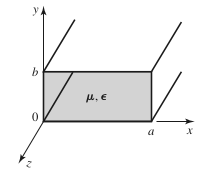
\includegraphics[scale=0.6]{rectangular}
  \caption{Guia d' ona rectangular}
  \label{rectangular}
  \vspace{-1 em}
\end{figure}

\begin{equation}
  \label{otherfields}
  \vec e_t = \frac{- \jmath \beta}{k^2 - \beta ^2} \del _t  e_z \quad i \quad \vec h_t = Y_{TM} \uz \times \vec e_t
\end{equation}

Resolent \cref{ezhelm} per separació de les variables $x$ i $y$ obtenim
\begin{equation}
  e_z = \left[ A \cos (k_x x ) + B \sin (k_x x) \right ] \left[ C \cos(k_y y ) + Dsin(k_y y) \right]
\end{equation}

On $k_x ^2 + k_y ^2 = k^2 - \beta ^2$. Per a calcular $\beta$ usar les condicions de contorn, que són
\begin{equation}
  e_z(x = a) = e_z (x = 0) = e_z(y = b) e_z(y = 0) = 0
\end{equation}

De les dos primeres obtenim que $A = 0$ i $k_X = \frac{n \pi}{a}$, i de les dos segones $C = 0$ i $k_y = \frac{m \pi}{b}$, el que ens deixa
\begin{equation}
  \label{solez}
  e_z (x, y) = BD \sin \frac{n \pi}{a} \sin \frac{m \pi }{b} = E_0  \sin \frac{n \pi}{a} \sin \frac{m \pi }{b}
\end{equation}

on hem reanomenat el coeficient $BD$ com a $E_0$, i
\begin{equation}
  \label{eq:solbeta}
  \beta_{nm} = \sqrt{ \omega ^2 \mu \epsilon - k_x ^2 - k_y ^ 2 } = \sqrt{\omega^2 \mu \epsilon - \left (\frac{n \pi}{a} \right ) ^2 - \left ( \frac{m \pi}{b} \right) ^2 }
\end{equation}

Per a cada parella $(n, m)$ existeix una solució, o el que és el mateix, un mode $TM_{nm}$, (excepte per al cas $n=m=0$, ja que seria la solució trivial en que no hi ha camps). Per a que aquests modes es propaguen $\beta $ haurà de ser real, el que implica
\begin{equation}
  \label{conds}
  \omega ^2 \mu \epsilon >  \left (\frac{n \pi}{a} \right ) ^2  + \left ( \frac{m \pi}{b} \right) ^2
\end{equation}

Definim per tant la freqüència de tall del mode $TM_{nm}$ com
\begin{equation}
  \omega _{c \,nm} =  \frac{1}{\sqrt{\mu \epsilon}} \sqrt{   \left (\frac{n \pi}{a} \right ) ^2 + \left ( \frac{m \pi}{b} \right) ^2}
\end{equation}

on s' observa que a freqüències més altes més modes seran propagables. La resta de camps poden obtindre's usant \cref{otherfields}:
\begin{subequations}
\begin{align}
  \vec e_t = \frac{ - \jmath \beta }{k^ 2 - \beta ^ 2} E_0
  \bigg [
    &+\left (\frac{n \pi}{a} \cos \frac{n \pi x}{a} \sin \frac{m \pi y}{b} \right ) \ux \nonumber \\
    &+\left (\frac{m \pi}{b} \sin \frac{n \pi x}{a} \cos \frac{m \pi y}{b} \right )\uy
  \bigg ] \\
  \vec h _ t = \frac{  -\jmath \omega \epsilon }{k^ 2 - \beta ^ 2} E_0
  \bigg [
    &-\left (\frac{m \pi}{b} \sin \frac{n \pi x}{a} \cos \frac{m \pi y}{b} \right ) \ux \nonumber \\
    &+\left (\frac{n \pi}{a} \cos \frac{n \pi x}{a} \sin \frac{m \pi y}{b} \right ) \uy
  \bigg ]
\end{align}
\label{rectTM}
\end{subequations}

El procediment amd els modes $TE$ és anàleg, usant les condicions de contorn
\begin{equation}
  \vec h_t = 0 \to \left. \del h_z \right \vert \sub{parets} = 0 \to \left. \pd{h_z}{x}  \right \vert \sub{par} =  \left. \pd{h_z}{y}  \right \vert \sub{par} = 0
\end{equation}
obtenim
\begin{equation}
  h_z = H_0 \cos \left ( \frac{n \pi x}{a} \right ) \cos \left ( \frac{m \pi y}{b} \right )
\end{equation}
\begin{subequations}
\begin{align}
  \vec h_t = \frac{  \jmath \beta }{k^ 2 - \beta ^ 2} H_0
  \bigg [
    &+\left (\frac{n \pi}{a} \sin \frac{n \pi x}{a} \cos \frac{m \pi y}{b} \right ) \ux + \nonumber \\
    &+\left ( \frac{m \pi }{b} \cos \frac{n \pi x}{a} \sin \frac{m \pi y}{b} \right ) \uy
  \bigg ] \\
  \vec e _ t = \frac{  \jmath \omega \mu }{k^ 2 - \beta ^ 2} H_0
  \bigg [
    &+\left (\frac{m \pi}{b} \cos \frac{n \pi x}{a} \sin \frac{m \pi y}{b} \right ) \ux \nonumber \\
   &-\left ( \frac{n \pi }{a} \sin \frac{n \pi x}{a} \cos \frac{m \pi y}{b} \right ) \uy 
  \bigg ]
\end{align}
\end{subequations}

amb
\begin{equation}
  \beta = \sqrt{ \omega ^2 \mu \epsilon - k_x ^2 - k_y ^ 2 } = \sqrt{\omega^2 \mu \epsilon - \left (\frac{n \pi}{a} \right ) ^2  - \left ( \frac{m \pi}{b} \right) ^2 }
\end{equation}
\begin{equation}
  \omega _{c \,nm} =  \frac{1}{\sqrt{\mu \epsilon}} \sqrt{   \left (\frac{n \pi}{a} \right ) ^2 + \left ( \frac{m \pi}{b} \right) ^2}
\end{equation}

\begin{figure}[ht]
\begin{minipage}{8cm}
  \centering
  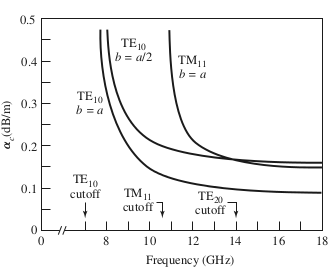
\includegraphics[scale=0.5]{rectangularmodes}
  \caption{Atenuació de modes en una guia rectangular}
  \vspace{-1 em}
\end{minipage}
\begin{minipage}{8cm}
  \centering
  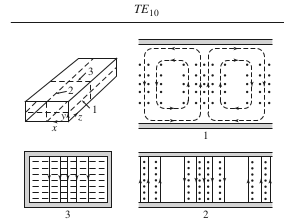
\includegraphics[scale=0.6]{rectangularfundamental}
  \caption{Mode fonamental d' una ona rectangular}
  \label{rectangularfundamental}
  \vspace{-1 em}
\end{minipage}
\end{figure}

\section{Mode fonamental}

El mode fonamental és aquell que es propaga amb la menor freqüència de tall. En el cas de la guia rectangular és el $TE_{10}$, graficat en la figura \cref{rectangularfundamental}
\begin{equation}
  \vec E = - H_0 \frac{\jmath \omega \mu a}{\pi} \sin \left ( \frac{\pi}{a} x \right) \uy
\end{equation}
\begin{equation}
  \vec H =  H_0 \left[\frac{\jmath \beta a}{\pi} \sin \left ( \frac{\pi}{a} x \right) \ux + \cos \left ( \frac{\pi}{a} x \right ) \uz \right]
\end{equation}

\section{Guia circular}

Usarem la guia circular (figura \cref{circular}) per a il·lustrar el cas en que la simetria fa preferible utilitzar coordenades no cartesianes, en aquest cas les cilíndriques $(s, \varphi, z)$.

Per a trobar els modes $TM_{nm}$ resolem, com abans, l' equació de Helmholtz, però aquesta vegada usant el Laplacià en coordenades cilíndriques:
\begin{equation}
  \del _t ^ 2 e_z + (k^ 2 - \beta ^2 ) e_z = \left ( \pd[2]{}{s} + \frac{1}{s}\pd{}{s} + \frac{1}{s^2} \pd[2]{}{\varphi}  \right )  e_z + k_c ^2 e_z
\end{equation}

\begin{figure}[ht]
  \centering
  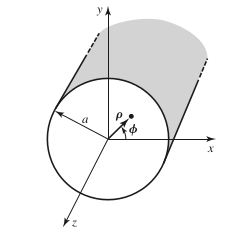
\includegraphics[scale=0.4]{circular}
  \caption{Guia d' ona circular}
  \label{circular}
  \vspace{-1 em}
\end{figure}

Separant $e_z$ en $R(s)\Phi(\varphi)$ arribem a dues equacions:
\begin{equation}
  \frac{s^2}{R(s)} \pd[2]{R}{s} + \frac{s}{R(s)} \pd{R}{s} + (k^2 - \beta ^2) s^2  =
  \frac{1}{\Phi(\varphi)} \pd[2]{\Phi}{\varphi} =
  k_{\varphi} ^2
\end{equation}

Ls solucions de la part angular són simples:
\begin{equation}
  \label{solangular}
  \Phi (\varphi) = A \cos(k _{\varphi} \varphi ) + B \sin (k_{\varphi} \varphi)
\end{equation}
però les de la part radial són més complicades; són funcions de Bessel primer i segon espècie:
\begin{subequations}
  \begin{align}
    R(s) = \Bf _{k_\varphi} (s\sqrt{k^2 - \beta ^2})  =  \Bf _{k_\varphi} (s k_c)  \nonumber \\
    R(s) = \Bs _{k_\varphi} (s\sqrt{k^2 - \beta ^2})  =  \Bs _{k_\varphi} (s k_c)  \nonumber
  \end{align}
\end{subequations}

Com que el camp ha de ser continuu en la coordenada angular tenim la condició de contorn
\begin{equation}
  e_z(\varphi = \alpha) = e_z ( \varphi = \alpha + 2 \pi l) \quad \forall \alpha \quad \forall l \in \Nat
\end{equation}

que, introduïda en \cref{solangular} ens diu que $k_{\varphi} \in \Zahl$:
\begin{equation}
  \Phi (\varphi ) = A \cos (n \varphi ) + B \sin (n \varphi)
\end{equation}

En quant a la part radial, en $s = 0$ les funcions de Bessel de segon espècie $\Bs$ divergeixen, pel que $D = 0$, i la condició de contorn de les parets $e_z(s = 0) = a$, que ha de cumplir-se $\forall \varphi$ ens dona el valor de $k_c$ per al mode $n$: és la solució de
\begin{equation}
  \Bf _ n (k_c a ) = 0
\end{equation}

Com que les funcions $\Bf$ no tenen arrels analítiques haurem d' utilitzar taules o procediments numèrics per trobar-les. Denotarem la $m$-èsima arrel de $\Bf$ com a $P_{nm}$, i per tant $k_c = \frac{P_{nm}}{a}$. La solució final, doncs, és (anomenem $AC = E$ i $BC = F$):
\begin{equation}
  e_z = E \cos (n \varphi ) \Bf _n ( \frac{P_{nm}}{a} s ) + F \sin (n \varphi ) \Bf_n (\frac{P_{nm}}{a}s)
\end{equation}
amb $ \beta = \sqrt{\omega ^ 2 \mu \epsilon - \left ( \frac{P_{nm}}{a} \right ) ^2}$.

Tenim dos coeficients independents perquè hi ha dos graus de llibertat al sistema: la energia de la ona i la polarització d' aquesta. Rotant el sistema de coordenades podem fer zero una o l' altra. Obtindre la resta dels camps, com abans, és un procediment mecànic:
\begin{subequations}
  \begin{align}
    \vec e_t =& -\frac{\jmath \beta}{k^2 - \beta ^2} \del _t  e_z =  \vec e_t = \frac{- \jmath \beta}{k^2 - \beta ^2} \left ( \pd{ e_z}{s} \us + \frac{1}{s} \pd{e_z}{\varphi} \uf \right ) \nonumber \\
    =& \left(-\frac{ \jmath \beta}{k_c} \left [ E \cos (n \varphi) + F \sin (n \varphi) \right ] \Bf _n ' \left( \frac{P_{nm}}{a} s \right) \right) \us  \nonumber\\
     & \left(-\frac{ \jmath \beta }{k_c ^2 } \frac{n}{s} \left [ E \sin (n \varphi) - F \cos (n \varphi) \right ] \Bf _n \left(\frac{P_{nm}}{a} s \right) \right) \uf \\
    \vec h_t =& \, Y_{TM} \uz \times \vec e_t \nonumber \\
    =& \left( -\frac{ \jmath \omega \epsilon}{k_c^2} \frac{n}{s} \left [ E \sin (n \varphi) - F \cos (n \varphi) \right ] \Bf _n \left( \frac{P_{nm}}{a} s \right) \right) \us  \nonumber \\
     & \left (-\frac{ \jmath \omega \epsilon }{k_c } \left [ E \cos (n \varphi) + F \sin (n \varphi) \right ] \Bf _n '\left(\frac{P_{nm}}{a} s \right) \right ) \uf
  \end{align}
  \label{circTM}
\end{subequations}

\begin{figure}[ht]
\begin{minipage}{8cm}
  \centering
  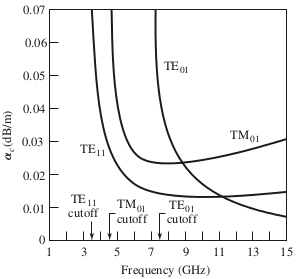
\includegraphics[scale=0.5]{circularmodes}
  \caption{Modes en una guia circular}
  \vspace{-1 em}
\end{minipage}
\begin{minipage}{8cm}
  \centering
  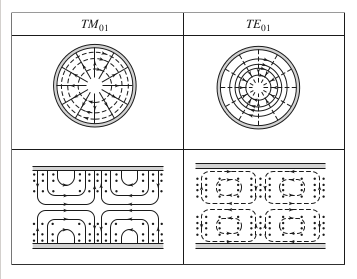
\includegraphics[scale=0.5]{circularmodesshape}
  \caption{Modes en una guia circular}
  \vspace{-1 em}
\end{minipage}
\end{figure}

\section{Guia coaxial}

La guia coaxial és una línia de transmissió que té moltes aplicacions gràcies al seu gran ample de banda, la seua baixa atenuació, i la capacitat de protegir les senyals propagades d' interferències exterior. En principi està dissenyada per a transmetre modes $TEM$, i podem utilitzar l' anàlisis del capítol 2, però és interessant estudiar el comportament dels camps d' aquesta quan transporta modes $TE$ o $TM$, ja que de vegades és inevitable que aquests modes apareguen junt al $TEM$ quan treballem amb freqüències altes (superiors a la del mode fonamental) o quan hi ha discontinuïtats, i és necessari saber com evitar interferències.

\begin{figure}[ht]
  \centering
  \begin{minipage}{7cm}
    \centering
    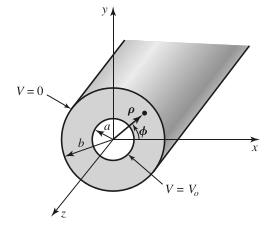
\includegraphics[scale=0.4]{coaxial}
    \caption{Guia d' ona coaxial}
    \label{coaxial}
  \end{minipage}
  \begin{minipage}{7cm}
    \centering
    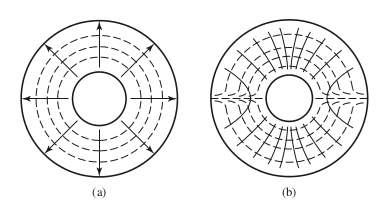
\includegraphics[scale=0.4]{coaxialmodes}
    \caption{Modes en una ona coaxial}
  \end{minipage}
\end{figure}

Quan apareixen aquestes discontinuïtats? Quan una guia s' estreta pot donar-se el cas que el mode fonamental es talle més enllà d' aquest punt, i la energia de la ona es reflectisca. Si després d' una distància curta l guia es torna a eixamplar és possible que el mode fonamental original torne a propagar-se. Que estiga tallat vol dir que s' atenua exponencialment, així que si no hi ha suficient distància per a que s' extingisca completament existirà un camp harmònic al final de la discontinuïtat, com si hi haguera un generador \footnote{En termes de fotons aquestes dos situacions són equivalents a un fotó rebotant contra una pared potencial infinita i fent efecte tunel, respectivament.}. Aquest fenomen pot ser usat per a excitar cavitats: necessitem fer entrar una ona en una regió tancada, però si fem un forat massa gran la cavitat tindrà massa pèrdues.

\subsection{Modes TE}

Com en el cas anterior comencem resolent l' equació de Helmholtz per a $h_z$ en coordenades cilíndriques, i després obtenim $\vec h_t$, $\vec e_t$ i $\beta$. Les solucions per a $h_z$ són, com abans,
\begin{equation}
  \Phi = A \cos ( n \varphi) + B \sin (n \varphi)
\end{equation}
\begin{equation}
  R = C \Bf_n ( k_c s ) + D \Bs_n (k_c s)
\end{equation}


On ja hem aplicat la continuïtat de la coordenada angular $\Phi(\varphi) = \Phi(\varphi + 2\pi l)$. Ara, però, no podem utilitzar la condició de contorn en $s = 0$ que hem utilitzat amb la guia circular, ja que ara el punt $s = 0$ no és part del problema, i $\Bs$ no divergeix. Per a traure els coeficients usarem les condicions de continuïtat de $h_t$ a les parets: la component radial ha d' anul·lar-se a les parets. Com que $h_t \propto \del h_z$ podem dir que
\begin{equation}
   \left. \pd{h_z}{s} \right \vert \sub{parets} = 0 \quad \to \quad \left. \pd{R}{s} \right \vert \sub{s = a} = \left. \pd{R}{s} \right \vert \sub{s = b} = 0
\end{equation}

Amb el que arribem a un sistema d' equacions en les incògnites C i D
\begin{equation}
  C\Bf _n ' (k_c a) + D \Bs _ n ' (k_c a) = 0
\end{equation}
\begin{equation}
  C\Bf _n ' (k_c b) + D \Bs _ n ' (k_c b) = 0
\end{equation}

Per a que existisca una solució el determinant de la matriu de coeficients ha de ser zero, i per tant hem de tindre
\begin{equation}
  \Bf _n ' (k_c a) \Bs _n ' (k_c b ) - \Bf _n ' (k_c b) \Bs _n ' (k_c a) = 0
\end{equation}

Cada solució numèrica $m$ d' aquesta equació transcendental proporciona, per al mode $n$, una $k_{c\,nm}$. Els coeficients $C$ i $D$ no són independents; estan lligats per
\begin{equation}
  \frac{C}{D} = -\frac{\Bf _n ' (k_c b )}{\Bs _n ' (k_c b )} = -\frac{\Bf _n ' (k_c a )}{\Bs _n ' (k_c a )}
\end{equation}

La solució per al camp axial queda
\begin{equation}
  h_z = [A \cos (n \varphi) + B \sin (n \varphi) ][C \Bf _n ' (k_c \varphi) + D \Bs _n ' (k_c \varphi)]
\end{equation}

i els camps transversals es poden obtenir pel mètode habitual.


\section*{Nota}

Pareix que sempre que utilitzem coordenades cilíndriques pugam utilitzar la condició de continuïtat de $\varphi$, però en realitat no és questió del sistema de coordenades utilitzat, sino de la guia, que té simetria angular. Hi ha casos en que no hi ha aquesta simetria, per exemple en una guia amb secció en forma de "formatget". En aquest cas, però, tindriem CC en $\varphi=0$ i $\varphi = \alpha$.